\section{Wahrscheinlichkeitsrechnung}
  \subsection{Begriffe}
  \textbf{Ergebnisraum} $\Omega$: Menge aller möglichen Ergebnisse eines Experiments\\
  \textbf{Elementarereignis} $\omega \in \Omega$: einzelnes Element von $\Omega$\\
  \textbf{Ereignis}$E \subseteq \Omega$: beliebige Teilmenge des Ergebnisraums $\Omega$ heißt sicheres Ereignis, $\emptyset$ heißt unmögliches Ereignis\\
  \textbf{Vereinigung} $E \cup F$: Ereignis E oder Ereignis F treten ein. $\bigcup_{i=1}^{n} E_{i}$: mindestens ein Ereignis $E_{i} $tritt ein.\\
  \textbf{Schnitt} $E \cap F$: Ereignis E und Ereignis F treten ein.\\
  $\bigcap_{i=1}^{n} E_{i}$ alle Ereignisse $E_{i}$ treten ein.
  \textbf{Gegenereignis} $\overline{E} = \Omega /\ E$: Ereignis E tritt nicht ein (Komplement von E)\\
  \textbf{Disjunkte Ereignisse}E  und F: $E \cap F = \emptyset$
  \subsection{De Morgan'schen Regeln}
  $\overline{E_{1} \cup E_{2}} = \overline{E}_{1} \cap \overline{E}_{2}$\\
  $ \overline{E_{1} \cap E_{2}} = \overline{E}_{1} \cup \overline{E}_{2}$
  \subsection{Wahrscheinlichkeit}
  $0 \le P(E) \le 1$; P($\Omega$) = 1;\\
  P($\bigcup_{i=1}^{\infty}) = \sum_{i=1}^{\infty}$ P($E_{i}$), falls $E_{i} \cap E_{j} = \emptyset$ für $i \neq j$\\
    \subsubsection{Satz 2.1}
    P($\overline{E}$) = 1 -P(E)\\
    P($E \cup F$) = P(E)+ P(F) - P($E \cap F$)
  \textbf(Übungsaufgabe!!! Ergänzen)\\
  \subsection{Laplace-Experiment}
  Zufallsexperimente mit n gleich wahrscheinlichen Elementarereignissen. Dann berechnet sich die Wahrscheinlichkeit P(E) für $E \subseteq \Omega$ aus:\\
  P(E) =$\frac{Anzahl der für E günstigen Ereignisse}{Anzahl der möglichen Ereignisse} = \frac{Mächtigkeit von E}{Mächtigkeit von \Omega} = \frac{|E|}{\Omega}$
  \textbf{text}
  \subsection{Kombinatorik}
  \subsubsection{Allgmeines Zählprinzip}
  Anzahl der Möglihckeiten für ein k-stufiges Zufallsexperiment mit $n_{i}$ Varianten im i-ten Schritt:
  $n_{1} \cdot n_{2} \cdot \text{...} \cdot n_{k}$
  \subsubsection{Permutationen}
  Anzahl einer n-elementigen Menge n-maliges Ziehen ohne Zurücklgen mit Beachtung der Reihenfolge: \textbf{n unterscheidbare Elemente}: $n! = n \cdot(n-1) textbf{...} 2 \cdot 1$
  \textbf{k Klassen mit je $n_{i}$ nicht unterscheidbaren Elementen} $n = sum_{k }^{i=1} n_{i}$:
  $\frac{n!}{n_{1}! \cdot n_{2}!\cdot \text{...}n_{k}! }$
  \subsubsection{Anzahl k-elementigen Teilmengen einer n-elementigen Menge k-maliges Ziehen aus einer n-elementigen Menge}
  ohne Zurücklegen = $k\le n$.\\
  mit Zurücklegen = $ k > n$ möglich.\\
  \textbf{mit Beachtung der Reihenfolge, ohne Zurücklegen}: $\frac{n!}{(n-k)!}$\\
  \textbf{ohne Beachtung  der Reihenfolge, ohne Zurücklegen}: $\binom{n}{k} = \frac{n!}{(n-k)! k!}$\\
  \textbf{mit Beachtung der Reihenfolge, mit Zurücklegen}: $n^k$\\
  \textbf{ohne Beachtung der Reihenfolge, mit Zurücklegen} $\binom{n+k-1}{k}$
  \subsection{Bedingte Wahrscheinlichkeit}
  $P(E|F) = P_{F}(E) = \frac{|E \cap F| }{|F|} = \frac{P(E\cap F))}{P(F)}$
  \subsubsection{Satz 2.2}
  $P(E \cap F) = P(E|F) \cdot P(F)$\\
  $P(E \cap F) = P(F|E) \cdot P(E)$\\
  	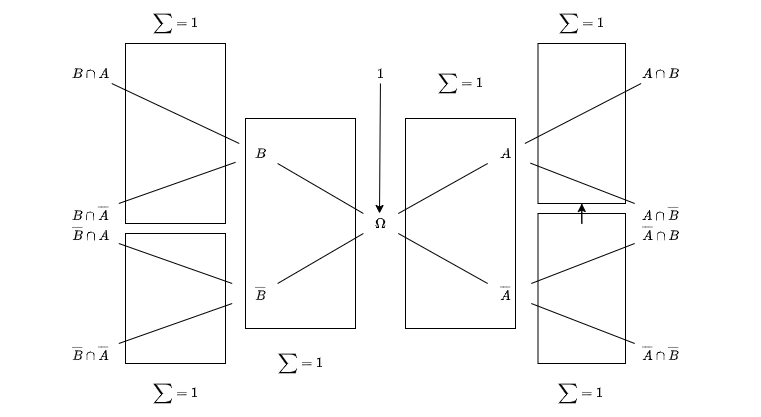
\includegraphics[scale=0.2]{./pic/BedingteWahrscheinlichkeit.png}
  	\subsubsection{Satz der totalen Wahrscheinlichkeit}
  	Sei $\Omega = \bigcup_{i=1}^{n} E_{i}$ mit $E_{i} \cap E_{j} =  \varnothing$ für $i \ne j$ d.h. die Ereignisse bilde eine disjunkte Zerlegung bzw. eine Partition von $\Omega$. Somit gilt:\\
  	$P(F) = \sum_{i=1}^{n} P(F \cap E_{i}) = \sum_{i=1}^{n} P(F|E_{i}) \cdot P(E_{i})$\\
  	Summe der Äste des Wahrscheinlichkeitsbaums zu allen Schnitten $F \cap E_{i}$
  	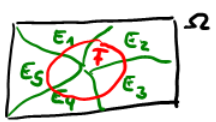
\includegraphics[scale=0.25]{./pic/SatzTotalerWahrscheinlichkeit.png}
  	\subsubsection{Vierfeldertafel}
  	$P(F) = P(F \cap E ) + P(F \cap \overline{E})$\\
  	$P(\overline {F}) = P(\overline{F} \cap E) + P(\overline{F} \cap E)$\\
  	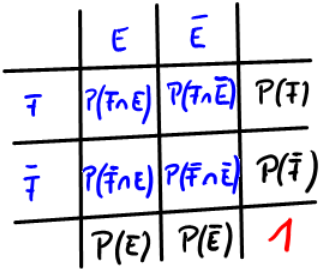
\includegraphics[scale=0.25]{./pic/Vierfeldertafel}
  	\textbf{Satz 2.2}
  	$P(E \cap F)  P(E) \cdot P(F|E) = P(F) \cdot P(E|F) $
  	\textbf{Tafel}
  	$= P(F) - P(F \cap \overline{E})$
  	$ = P(E) - P(\overline{F} \cap E)$; 
  $P(\overline{F} | E) = 1 - P(F | E)$
  \subsubsection{Formel von Bayes}
  Hilfreich, wenn man man $P( F | E_{i} )$ kennt, aber nicht $P(E_{k}|F)$
  \textbf{Satz 2.4}
  $P(E_{k} | F) = \frac{ P(F | E_{k}) \cdot P(E_{k})}{ \underbrace{\sum_{i=1}^{n}P(F|E_{i}) \cdot P(E_{i})}}$\\
\textbf{Nur Nenner!}P(F) aus dem Satz der totalen Wahrscheinlichkeit.
  \subsubsection{Stochastische Unabhängigkeit}
  \textbf{Uebung}
  Die Ereignisse E und F heißen (stochastisch) unabhängig, wenn die Information über das Eintreten des einen Ereignisses die Wahrscheinlichkeit für das Eintreten des anderen Ereignisses nicht ändert, d.h. falls\\
  $\underbrace{P(E|F)}= P(E) oder P(E\cap F) = P(E) \cdot P(F)$\\
  $= \frac{P(E \cap F)}{P(F)}$\\
  \textbf{Es gilt}
  Falls die Ereignisse E, F unabhängig sind, dann sind auch:\\
  \subitem $E, \overline{F}$
  \subitem $\overline{E} , F$
  \subitem $\overline{E}, \overline{F}$
  unabhängig
  \textbf{Bemerkung}
  \begin{itemize}
  	\item Stochastische Unabhängigkeit bedeutet nicht notwendigerweise eine kausale Abhängigkeit
  	\item Veranschaulichung mit Venn Diagramm
  	  \includegraphics[scale=0.23]{./pic/StochastischeUnabhängigkeit.png}
  	  \includegraphics[scale=0.23]{./pic/StochastischeAbhängigkeit.png}
  	\item $A, B \ne \varnothing$ und $A \cap B  = \varnothing$\\
  	$P(A\cap B) \stackrel{?}{=} P(A) \cdot P(B)$\\
  	$\varnothing \ne P(A) \cdot P(B)$ da P(A) > 0 und P(B)> 0\\
  	=> A, B stochastisch abhängig
  \end{itemize}
  
  